\documentclass{article}%
\usepackage[T1]{fontenc}%
\usepackage[utf8]{inputenc}%
\usepackage{lmodern}%
\usepackage{textcomp}%
\usepackage{lastpage}%
\usepackage[tmargin=1cm,bmargin=2cm,lmargin=1cm]{geometry}%
\usepackage{multicol}%
\usepackage{graphicx}%
\usepackage{adjustbox}%
\usepackage{tkz-euclide}%
\usepackage{amsmath}%
\usepackage{scalefnt}%
\usepackage{enumitem}%
%
%
%
\begin{document}%
\normalsize%
\setlength\itemsep{-2cm}%
\section{Write the equation of a line given the slope and y{-}intercept (Challenge)}%
\label{sec:Writetheequationofalinegiventheslopeandy{-}intercept(Challenge)}%
\textbf{Learning Goal: }\hrulefill \\ \hrulefill%
\begin{multicols}{2}%
\begin{enumerate}[label=\arabic*),start=1]%
\item\adjustbox{valign=t}{\begin{minipage}{\linewidth}
Write the equation of the line shown in the graph.\\

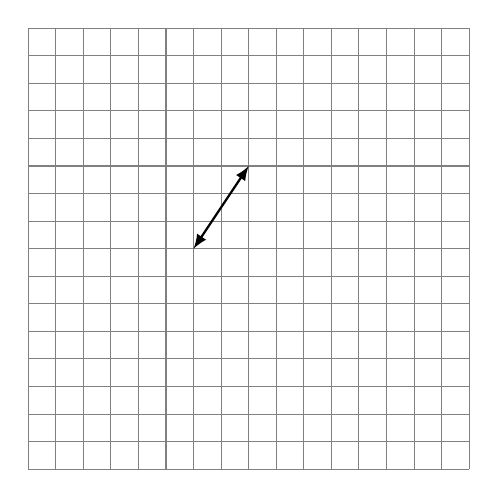
\begin{tikzpicture}[font=\tiny,scale=0.35]
   %\tikzstyle{every node}=[font=\small]
   \tkzInit[xmax=8,ymax=8,xmin=-8,ymin=-8]
   \tkzGrid
   \tkzAxeXY
   \draw[ thick,latex-latex] (0,3) -- (-2,0);% node[anchor=south west] {$a$}; % two points for drawing 2x+y=2
%  \tkzText[above](0,6.75){Desired Output}
  \end{tikzpicture}
\end{minipage}}%
\vspace{3cm}%
\item\adjustbox{valign=t}{\begin{minipage}{\linewidth}
Write the equation of the line with y-intercept $(0,-40)$ and slope $2$.\\

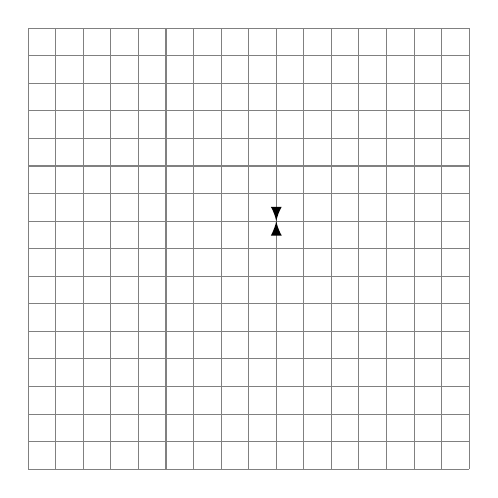
\begin{tikzpicture}[font=\tiny,scale=0.35]
   %\tikzstyle{every node}=[font=\small]
   \tkzInit[xmax=8,ymax=8,xmin=-8,ymin=-8]
   \tkzGrid
   \tkzAxeXY
   \draw[ thick,latex-latex] (,) -- (,);% node[anchor=south west] {$a$}; % two points for drawing 2x+y=2
%  \tkzText[above](0,6.75){Desired Output}
  \end{tikzpicture}
\end{minipage}}%
\vspace{0cm}%
\item\adjustbox{valign=t}{\begin{minipage}{\linewidth}
\\

%\vspace{4cm}

\begin{tikzpicture}[font=\small,scale=0.40]
   \tikzstyle{every node}=[font=\small]
   \tkzInit[xmax=6,ymax=6,xmin=-6,ymin=-6]
   \tkzGrid
   \tkzAxeXY
%   \draw[ thick,latex-latex] (-1,4) -- (4,-6) node[anchor=south west] {$a$}; % two points for drawing 2x+y=2
%  \tkzText[above](0,6.75){Desired Output}
  \end{tikzpicture}
\end{minipage}}%
\vspace{0cm}%
\item\adjustbox{valign=t}{\begin{minipage}{\linewidth}
\\

%\vspace{4cm}

\begin{tikzpicture}[font=\small,scale=0.40]
   \tikzstyle{every node}=[font=\small]
   \tkzInit[xmax=6,ymax=6,xmin=-6,ymin=-6]
   \tkzGrid
   \tkzAxeXY
%   \draw[ thick,latex-latex] (-1,4) -- (4,-6) node[anchor=south west] {$a$}; % two points for drawing 2x+y=2
%  \tkzText[above](0,6.75){Desired Output}
  \end{tikzpicture}
\end{minipage}}%
\vspace{0cm}%
\item\adjustbox{valign=t}{\begin{minipage}{\linewidth}
\\

%\vspace{4cm}

\begin{tikzpicture}[font=\small,scale=0.40]
   \tikzstyle{every node}=[font=\small]
   \tkzInit[xmax=6,ymax=6,xmin=-6,ymin=-6]
   \tkzGrid
   \tkzAxeXY
%   \draw[ thick,latex-latex] (-1,4) -- (4,-6) node[anchor=south west] {$a$}; % two points for drawing 2x+y=2
%  \tkzText[above](0,6.75){Desired Output}
  \end{tikzpicture}
\end{minipage}}%
\vspace{0cm}%
\item\adjustbox{valign=t}{\begin{minipage}{\linewidth}
\\

%\vspace{4cm}

\begin{tikzpicture}[font=\small,scale=0.40]
   \tikzstyle{every node}=[font=\small]
   \tkzInit[xmax=6,ymax=6,xmin=-6,ymin=-6]
   \tkzGrid
   \tkzAxeXY
%   \draw[ thick,latex-latex] (-1,4) -- (4,-6) node[anchor=south west] {$a$}; % two points for drawing 2x+y=2
%  \tkzText[above](0,6.75){Desired Output}
  \end{tikzpicture}
\end{minipage}}%
\vspace{0cm}%
\item\adjustbox{valign=t}{\begin{minipage}{\linewidth}
Write an equation to represent the table below.\\

    \begin{tabular}{ | c | c |}
    \hline
    x & y \\ \hline
    
        -1 & -5 \\
    
        0 & -2 \\
    
        2 & 4 \\
    
        4 & 10 \\
    
    \hline
    \end{tabular}
\end{minipage}}%
\vspace{6cm}%
\end{enumerate}

%
\end{multicols}%
\end{document}